\documentclass[a4paper, 11pt]{article}

\usepackage[english]{babel}
\usepackage{graphicx}
\usepackage{appendix}
\usepackage[round]{natbib}
\usepackage[usenames, dvipsnames]{color}
\usepackage{fancyhdr}
\usepackage{hyperref}
\hypersetup{
	pdfmenubar = true, 
	colorlinks = true,
	linkcolor = black}
\newcommand{\CITE}[1]{\citep{#1}}
\begin{document}
\bibliographystyle{plainnatnourl} %%Self made package derived from plainnat without url and doi
\title{Literature Review of RNA Decay}
\author{Sun Mai}
\date{27. November 2010 $\sim$ \today}
\maketitle

\pagestyle{fancy}
\fancyhead{}
\fancyhead[R]{\slshape \leftmark}
\fancyfoot[C]{\thepage}

\newpage
\tableofcontents

\newpage
\sloppy
\section{Overview}
	\subsection{The different pathways in RNA degradation}
		\paragraph{}In the most species studied, RNA degradation is governed by multiple mechanisms. There are four general pathways(Figure \ref{pathway}): the deadenylation dependent decapping followed by 5'$\rightarrow$ 3' degradation, or 3'$\rightarrow$ 5' degradation by exosome, the endonucleolytic digestion and special quality control pathways.
		\begin{figure}[h] 
		\centering
			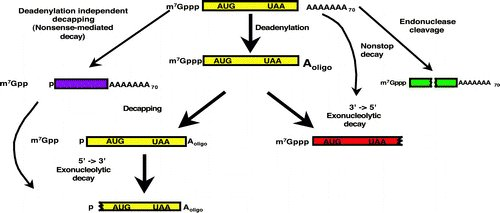
\includegraphics[scale=0.5]{pathway.jpg}
			\caption{The draft of different pathways of degradation\CITE{Coller2004}}
			\label{pathway}
		\end{figure}
		\paragraph{Degradation and translation are in competition}Translation competes with mRNA degradation \textit{in vivo}, some experimental results show this. For example mutations in translation initiation factors that decrease translation rates increase the rate of decapping\CITE{Schwartz1999}. All treatments that decrease ribosome loading increase decapping, whereas all manipulations that increase ribosome loading decrease decapping rates\CITE{LaGrandeur1999}. The tight association of the initiation complex with the cap can provide mRNA from decapping.
		\paragraph{Deadenylation leads to 5' $ \rightarrow $ 3' degradation}In yeast polyA shortening leads to decapping and thereby exposing the RNAs to 5' $\rightarrow $ 3' digestion by exonuclease\CITE{Muhlrad1994,Decker1993}. \textit{In vivo} the mRNAs is protected from decapping through a poly(A) dependent manner\CITE{Caponigro1995, Decker1993}. The poly(A) binding protein Pab1p plays the major role in the inhibition of decapping\CITE{Caponigro1995}.  The ability of Pab1p to inhibit decapping is intrinsic and is independent of the binding to poly(A)\CITE{Coller1998}. Decapping is conserved throughout eukaryotic organisms. Evidence shows that in yeast the 5' $ \rightarrow $ 3' degradation following decapping is faster then the 3' $ \rightarrow $ 5' degradation. However in some yeast mRNA 3' $ \rightarrow $ 5' degradation will be the dominant decay mechanism.
		\paragraph{Quality control pathways}The mRNAs which have premature stop codon triggers the NMD pathway. Or if the mRNA molecules lack a stop codon, they will be subjected to the non-stop decay. In both these cases, the mRNAs are targeted to cytoplasmic exosome by a special factor Ski7p. In nucleus, the RNAs which failed to be processed properly is also degraded by the nuclear exosome or the nuclear homologue of Xrn1p, the Rat1p.
\section{Deadenylation machinery and regulation}
	\subsection{Poly(A) binding protein Pab1p}
		\paragraph{Pab1p functions as negative regulator of RNA decay}mRNA is subjected to degradation when the poly(A) tail is shortened to certen length. Pab1p bind to poly(A) tail and inhibit both poly(A) shortening\CITE{Tucker2002} and decapping\CITE{Coller1998}.
	\subsection{Ccr4-Not complex}
		\paragraph{General about Ccr4-Not complex}Ccr4-Not complex is one of the global regulator of gene expression\CITE{Collart2003}. It regulates the RNA turnover at several steps. This multifunctional complex in \textit{S. cerevisiae} exists in two forms, one is the 0.9-1.2MDa complex, the other is the 1.9-2MDa, which contains proteins from the transcription machinary\CITE{Bai1999}. Ccr4-Not complex was identified as transcription factor, is important in the regulation of TFIID distribution on promoters\CITE{Lenssen2007, Lenssen2005}. Because the two subunits of this complex, Ccr4p and Caf1p, are deadenylases\CITE{Tucker2001}, Ccr4-Not complex also contributes to mRNA degradation. Ccr4-Not complex even has function in protein degradation, since Not4p was identified as a E3 ligase\CITE{Albert2002}.Latest study \textit{in vitro} confirmed Ccr4-Not complex function in transcription elongation\CITE{Kruk2011} by performing ChIP assay. Ccr4 is also found in the Cdc73p-Paf1p-Pol II-containing complex (Paf1p complex) also includes Ctr9p, Rtf1p, Leo1p, Gal11p, Ccr4p, Hpr1p, and the general initiation factors TFIIB and TFIIF, but lacks Tbp1p, TFIIH, and transcription elongation factor TFIIS, as well as the SRBps \\
		Ccr4-Not complex is structurally and functionaly divided into two modules, the Ccr4-Pop2 module and the Not2-Not5 module. The former one conducts the exnuclease activity \textit{in vivo}, whereas the latter one take part in transcription repression, protein degradation and etc. \\
		A detailed table contains the mutants studied is given in the ref. \CITE{Collart2003}
		\paragraph{Ccr4p} Ccr4p is 3'-exoribonuclease with a preference of poly(A)-substrate. The yeast Ccr4p contains 3 functional domains: the N-terminal extension, which is unique in \textit{Saccharomyces cerevisiae} and not found in higher eukaryotes; the central leucine-rich repeat(LRR), which is important for the contact between Ccr4p and Pop2p; and the C-terminal nuclease domain.
		\paragraph{Pop2p/Caf1p} Pop2p is one of the two catalytic subunits in Ccr4-Not complex\CITE{Tucker2001}. Pop2p belongs to the DEDD nuclease family, and shows 3'$\rightarrow$ 5' exnuclease activity with preferences for poly(A) sequence \textit{in vitro}. However, mutations of Pop2p to disrupt the catalytic activity doesn't cause deadenylation defect in \textit{in vivo}. Partial disruption of Pop2p inhibits the association of CCR4 with the NOT1 and NOT2 proteins\CITE{Liu1998, Bai1999}. Besides the structural function of Pop2p as a remainder of Ccr4-Not complex, it also has other separate functions in deadenylation \textit{in vivo}\CITE{Ohn2007}. Deadenylation end point defect is observed in several Pop2p mutants, in which conserved region is mutated or deleted\CITE{Ohn2007}. Furthermore, $\Delta$pop2 was shown synthetic lethal with $\Delta$dhh1, whereas $\Delta$ccr4 is not synthetic lethal with $\Delta$dhh1\CITE{Maillet2002}.
	\subsection{Pan2p/Pan3p exonuclease represents as second mRNA deadanylase}
\section{Decapping machinery and its regulation}
	\subsection{Dcp1p and Dcp2p}
		\paragraph{}Many experiment evidences show that the Dcp2p is the catalytic subunit of decapping machinery, whereas Dcp1p functions to enhance the activity of Dcp2p. Dcp2p contains a NUDIX/MutT domain, which's deletion leads to inactivation of Dcp2p \textit{in vivo} and \textit{in vitro}\CITE{Dunckley1999}. The activity of Dcp1/Dcp2p is not inhibited by cap analogues. This and other evidences suggest that the Dcp1/Dcp2p may bind to mRNA and this may allosterically regulate decapping activity.
	\subsection{The scavenger decapping enzyme DcpS}
		\paragraph{}There is another type of decapping enzyme, which degradate the short capped RNA produced by exosome dependent 5'$\rightarrow $3' degradation\CITE{Wang2001}. Long RNA substrate cannot be degraded by DcpS. It also hydrolyses the 7mGDP to produce 7mGMP and phosphate. The DcpS is a HIT domain contained protein, and it reacts specifically with methylated cap analogue \textit{in vitro}. It cannot hydrolyze unmethylated cap and intact capped RNA\CITE{Liu2002}.
	\subsection{The regulator of decapping}
		\paragraph{} The decapping process is regulated by both inhibition and enhancement. An example is the polyA binding protein Pab1p, deletion of Pab1p cause decapping prior to deadenylation\CITE{Caponigro1995, Morrissey1999}. Other proteins which bind to the the cap like eIF4E also inhibits the decapping. There are several groups of proteins, which play the role of enhancer of decapping.% still to be extended 
		\paragraph{Dhh1p}The decapping activatior Dhh1p and Pat1p function in the pathway of moving mRNAs from polysomes into the translationally inert state that accumulates in P bodies(Figure \ref{pbody}). Dhh1p and Pat1p interact with subunits in translation initiation complex, and repress translation, thus promote the P body formation. In study of glucose starvation, translational repression is observed in WT cell to response to the environment cue. But in \textit{dhh1}$\Delta$ and \textit{pat1}$\Delta$ strain, translational repression is only slightly impaired. Dhh1p represses translation may function in a way that Dhh1p directly binds to translation initiation factors. Experiments show that Dhh1p inhibits the formation of 48S complex \textit{in vitro}\CITE{Coller2005}. Dhh1p enhances the decapping event in the deadenylated mRNA, since in the \textit{dhh1}$\Delta$ strain, capped mRNA lacking polyA tail is accumulated, and impaired Dhh1p does not affect the mRNA deadenylation rate. Experiments also showed that, Dhh1p is not required for the NMD pathway \CITE{Fischer2002, Coller2001}. 
		\paragraph{Pat1p}Pat1p is topoisomerase II-associated deadenylation-dependent mRNA-decapping factor; also required for faithful chromosome transmission, maintenance of rDNA locus stability, and protection of mRNA 3'-UTRs from trimming; functionally linked to Pab1p. It contains a Pumilio domain and thus binds to mRNA. The confirmed binary interaction partners of Pat1p are Dhh1p, Lsm1p, Lsm2p, and Lsm4p.
		\begin{figure}[h] 
		\centering
			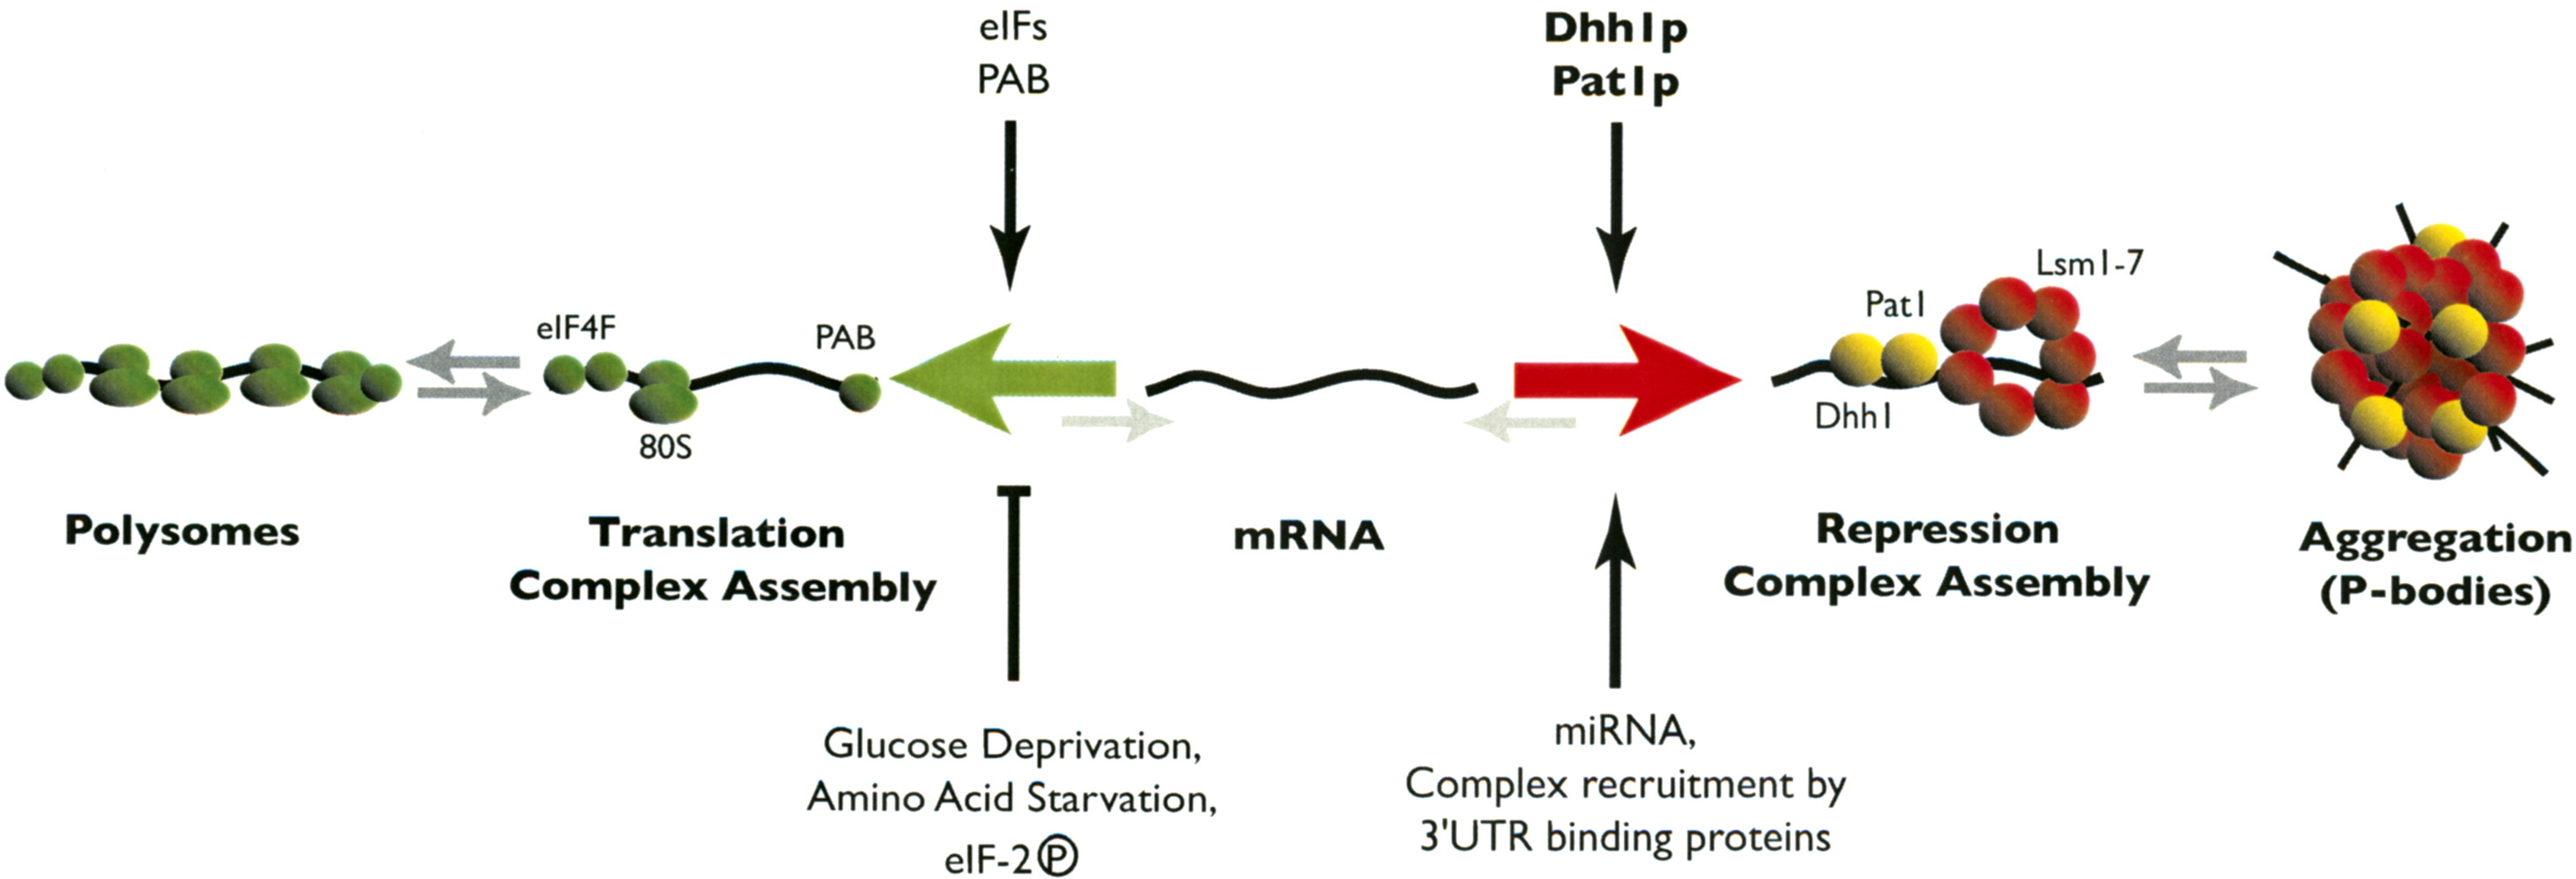
\includegraphics[scale=0.5]{Pat1pDhh1p.jpg}
			\caption{Model of the equilibrium shift between polysome formation and P body accumulation regulated by decapping activators and translation initiation factors\CITE{Coller2005}}
			\label{pbody}
		\end{figure}
		\paragraph{Edcs} The Edc1p and Edc2p proteins are identified as decapping enhancer since overexpression of them can compensate the synthetic lethality of temperature-sensitive allele of DCP1 and DCP2 and \textit{ski7}$\Delta$. They interact with Dcp1p and enhance the decapping activity. Edc1p and Edc2p bind to Dcp1, the general decapping activator, via its EVH1 domain, and thus enhance the decapping activity of Dcp2p by 1000-folds \CITE{Borja2011,SCHWARTZ2003}.
\section{5'$\rightarrow$3' degradation}	
	\subsection{Xrn1 and decapping dependent 5'$ \rightarrow $3' degradation}
		\paragraph{}The cap structure prevents mRNA from degradation, accumulation of mRNA without 5'-cap is observed in \textit{xrn1}$\Delta$ yeast\CITE{Hsu1993}. The exonuclease Xrn1p (or Kem1p in budding yeast) degrade preferentially mRNA with a 5'-mono-phosphate.
\section[The synthesis decay cross-talk]{The cross-talks between RNA decay, translation and transcription}
	\subsection{Cross-talk between RNA decay and translation}
	\subsection{P-body formation}
		\paragraph{Decapping occurs in P-body}In yeast, GFP-tagged Dcp1p, Dcp2p, Lsm1p, Pat1p, Dhh1p and Xrn1p have been localized to P bodies. When use the translation elongation inhibitor cycloheximide, which trap mRNA in polysomes, P bodies disappear in 10 min\CITE{Sheth2003}. This result strongly support the hypothesis that P bodies are the cellular foci, where decapping takes place. The existence of P bodies and that the mRNA are sequestrated into P bodies may suggest that it is a fundamental buffering system for translational control. Another explanation of the P body formation is because the high dynamic of mRNP. Because mRNP is highly dynamic, the mRNP binds to translation inhibitor can reenter the translation pool. Formation of a larger complex can make the ability to deliver the mRNA to the repressive center the rate-limiting step\CITE{Coller2004}.
		\\According to the model made by Franks and co-workers \CITE{Franks2008}, the P-body formation is via the homomeric interaction in prion-like domain of Lsm4p and Yjef-N domain of Edc3p.
	\subsection{Cross-talk between RNA decay and transcription}
	The study of enhanced ADH2 expression in \textit{spt10} strains leads to the fact, that affecting the mRNA transport and degradation can cause reduction of gene expression. This observation suggests that the transcription and RNA decay is interconnected \CITE{Denis2003}.
		\paragraph{The role of Rpb4/7 in mRNA decay and translation} Recent experiments show that the nonstoichiometric subunit Rpb4/7 bind to subunits of translation elongation factors, and thus affect the RNA stability by regulation translation initiation\CITE{Harel-Sharvit2010}. The results by studying the mutant Rpb6\textsuperscript{Q100R} which is reported to show poorly binding of Rpb4/7 to PolII, show that the recruitment of Rpb4/7 to polymerase is crucial in the regulation of translation. By studying the mutants altering the Rpb4/7 nuclear localization show that the shuttling of Rpb4/7 is necessity for the regulatory function of Rpb4/7 in translation.
\section{3' $\rightarrow$5' degradation}
	\subsection{The cytoplasmic exosome complex and its regulation}
		\paragraph{General introduction}
	\subsection{The nuclear exosome complex}
		\paragraph{The nuclear specific exosome subunit Rrp6p}
		\paragraph{The exosome associated RNA binding protein Rrp47}
\section{Regulation of the RNA stability by RNA binding proteins}
	\subsection{the Puf family}
		\paragraph{Puf4p and Puf5p negatively regulate mRNA by recruiting Ccr4-Not complex} Puf4p and Puf5p bind to 3'-UTR region of mRNA and stimulate deadenylation. This process requires physical interaction of Pop2p and the enzymatic activity of Ccr4p\CITE{Hook2007}.
		\paragraph{Puf proteins bind RNA using a ``two-handed'' mode} It is shown by systematic binding analysis, that each PUF protein yielded a similar binding pattern in which the central PUF repeats were less stringently required than those at the ends of the structure. Bases opposite amino acid residues that were less critical and all flipped bases generally were flexible in identity. These suggest a “two-handed” mode of recognition, in which interactions at the two ends of the complex are the most critical \CITE{Valley2012}. Human possess 2 different PUF proteins, the PUM1 and PUM2. They mediate translation inhibition in both deadenylation-dependent and independent mode\CITE{VanEtten2012}.
\section{Concerning the method}
	\subsection{Normalization with internal or external standard}
		\paragraph{Normalization with external standard} The idea of using external standard to monitor the global change of mRNA level was first brought out by Holstege and co-workers in the genome-wide study of artificial inactivation of RNA polymerase II \CITE{Holstege1998}. The method was described in detail in another paper \CITE{Peppel2003}. In this method, equal amount of external transcribed mRNAs are spiked into equal amount of total RNA (Figure \ref{normalization}). The cell number are counted, and the yield of total RNA is calculated respected to the cell number. Similar normalization method are also used in the study of RNA decay \CITE{Wang2002}. 
		\begin{figure}[h] 
		\centering
			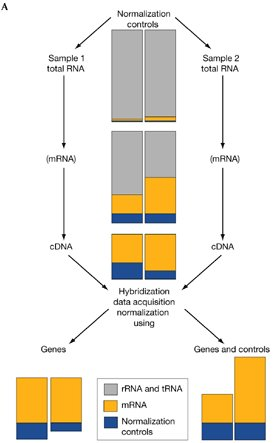
\includegraphics[scale=0.5]{Jeroen_2003_fig1.jpg}
			\caption{Normalization using external standard.\CITE{Peppel2003}}
			\label{normalization}
		\end{figure}

\newpage
\appendix
\section[Auxin-Degron strains]{Strains to be made use Auxin-Degron system}
	\paragraph{Positive control of this method} Because I modified the system the author used in the published work \CITE{Nishimura2009}, the modified system must be verified. In order to reproduce the effect that the author reported, IAA17-tag is made fusion to the gene Mcm4p ({\color{RoyalPurple}YPR019w}, which is the essential helicase component of heterohexameric MCM2-7 complexes which bind pre-replication complexes on DNA and melt the DNA prior to replication; accumulates in the nucleus in G1; homolog of S. pombe Cdc21p. 
	\subsection{The genes which are essential} Pab1 ({\color{blue}inviable}) Poly(A) binding protein, part of the 3'-end RNA-processing complex, mediates interactions between the 5' cap structure and the 3' mRNA poly(A) tail, involved in control of poly(A) tail length, interacts with translation factor eIF-4G 
\section[YKO strains]{Strains got directly from the YKO collection}
	\subsection{Deadenylation\CITE{Meyer2004}}
		\subsubsection{Ccr4p/Pop2p/Notp complex} Pop2/Caf1 ({\color{red}viable}) {\color{RoyalPurple}YNR052c} RNase of the DEDD superfamily, subunit of the Ccr4-Not complex that mediates 3' to 5' mRNA deadenylation(OpenBiosystem YKO collection No.: 7123)
		\\Ccr4 ({\color{red}viable}){\color{RoyalPurple}YAL021c} Component of the CCR4-NOT transcriptional complex, which is involved in regulation of gene expression; component of the major cytoplasmic deadenylase, which is involved in mRNA poly(A) tail shortening(OpenBiosystem YKO collection No.: 387) {\color{red}the strain was wrong, generated by us} 
		\\Caf40 ({\color{red}viable}) {\color{RoyalPurple}YNL288w} Evolutionarily conserved subunit of the CCR4-NOT complex involved in controlling mRNA initiation, elongation and degradation; binds Cdc39p(OpenBiosystem YKO collection No.: 1156)
\section[Genes involved in RNA turnover]{The complete list of the genes involved in RNA turnover}
	\subsection{Deadenylation\CITE{Meyer2004}}
		\subsubsection{Ccr4p/Pop2p/Notp complex} Pop2/Caf1 ({\color{red}viable}) {\color{RoyalPurple}YNR052c} RNase of the DEDD superfamily, subunit of the Ccr4-Not complex that mediates 3' to 5' mRNA deadenylation(OpenBiosystem YKO collection No.: 7123). Mutation S188A/E190A (\emph{according to the SGD annotation})of yeast Pop2 inactive Pop2p deadenylation activity \textit{in vitro}\CITE{Viswanathan2004}.
		\\Ccr4({\color{red}viable}){\color{RoyalPurple}YAL021c} Component of the CCR4-NOT transcriptional complex, which is involved in regulation of gene expression; component of the major cytoplasmic deadenylase, which is involved in mRNA poly(A) tail shortening(OpenBiosystem YKO collection No.: 387). The ccr4-2 mutant contains a single mutation(D713A) and is inactive \textit{in vitro}. It mediates elongated RNA halflife at some loci \textit{in vivo}\CITE{Chen2002}.
		\\Caf40 ({\color{red}viable}) {\color{RoyalPurple}YNL288w} Evolutionarily conserved subunit of the CCR4-NOT complex involved in controlling mRNA initiation, elongation and degradation; binds Cdc39p(OpenBiosystem YKO collection No.: 1156) 
		\\Caf130 ({\color{red}viable}) Part of the evolutionarily-conserved CCR4-NOT transcriptional regulatory complex involved in controlling mRNA initiation, elongation, and degradation 
		\\Caf120 ({\color{red}viable}) Part of the evolutionarily-conserved CCR4-NOT transcriptional regulatory complex involved in controlling mRNA initiation, elongation, and degradation 
		\\Caf16 ({\color{red}viable}) Part of evolutionarily-conserved CCR4-NOT regulatory complex; contains single ABC-type ATPase domain but no transmembrane domain; interacts with several subunits of Mediator 
		\subsubsection{Not multisubunit complex Not1-Not5} Not1(Cdc39) ({\color{blue}inviable}) Component of the CCR4-NOT complex, which has multiple roles in regulating mRNA levels including regulation of transcription and destabilizing mRNAs by deadenylation; basal transcription factor 
		\\Not2(Cdc36) ({\color{blue}inviable}) same as above \\Not3({\color{red}viable}) {\color{RoyalPurple}YIL038c} Subunit of the CCR4-NOT complex, which is a global transcriptional regulator with roles in transcription initiation and elongation and in mRNA degradation  (OpenBiosystem YKO collection No.: 1431) 
		\\Not4(Mot2) ({\color{red}viable}) {\color{RoyalPurple}YER068w} Subunit of the CCR4-NOT complex, which has roles in transcription regulation, mRNA degradation, and post-transcriptional modifications; with Ubc4p, ubiquitinates nascent polypeptide-associated complex subunits and histone demethyase Jhd2p (OpenBiosystem YKO collection No.: 207) 
		\\Not5 ({\color{red}viable}) {\color{RoyalPurple}YPR072w} Subunit of the CCR4-NOT complex, which is a global transcriptional regulator with roles in transcription initiation and elongation and in mRNA degradation (OpenBiosystem YKO collection No.: 5491)
		\vspace{6pt}
		\\Pan2 ({\color{red}viable}) {\color{RoyalPurple} YGL094c} Poly(A) ribonuclease, member of the PAN2p-PAN3p complex
		\\Pan3 ({\color{red}viable}) {\color{RoyalPurple} YKL025c} same as above 
		\\Pab1 ({\color{blue}inviable}) Poly(A) binding protein, part of the 3'-end RNA-processing complex, mediates interactions between the 5' cap structure and the 3' mRNA poly(A) tail, involved in control of poly(A) tail length, interacts with translation factor eIF-4G
		\vspace{6pt}
		\\Ngl1-3 ({\color{red}viable}) similar to Ccr4
	\subsection{Decapping}
	Dcp1 ({\color{blue}inviable}/{\color{red}viable}) {\color{RoyalPurple}YOL149w} Subunit of the Dcp1p-Dcp2p decapping enzyme complex, which removes the 5' cap structure from mRNAs prior to their degradation; enhances the activity of catalytic subunit Dcp2p; regulated by DEAD box protein Dhh1p. Ts-mutant\CITE{Dunckley2001} (dcp1-2: R29A, D31A), {\color{RoyalPurple}YOL149w}::kanMX4/{\color{RoyalPurple}YOL149w} strain: Y26658 on Euroscarf
	\\Dcp2 (inviable/viable) {\color{RoyalPurple}YNL118c} Catalytic subunit of the Dcp1p-Dcp2p decapping enzyme complex, which removes the 5' cap structure from mRNAs prior to their degradation; member of the Nudix hydrolase family Ts-mutant\CITE{Dunckley2001} (dcp2-7: N60D, I68V, D142V), {\color{RoyalPurple}YNL118c}::kanMX4/{\color{RoyalPurple}YNL118c} strain :Y22958 on Euroscarf \\Dcs1 ({\color{red}viable}) {\color{RoyalPurple}YLR270w} Non-essential hydrolase involved in mRNA decapping, may function in a feedback mechanism to regulate deadenylation, contains pyrophosphatase activity and a HIT (histidine triad) motif; interacts with neutral trehalase Nth1p (OpenBiosystem YKO collection No.: 5179)
	\vspace{6pt}
	\\Edc1 ({\color{red}viable}) {\color{RoyalPurple}YGL222c} RNA-binding protein, activates mRNA decapping directly by binding to the mRNA substrate and enhancing the activity of the decapping proteins Dcp1p and Dcp2p; has a role in translation during heat stress (OpenBiosystem YKO collection No.: 4588) 
	\\Edc2 ({\color{red}viable}) {\color{RoyalPurple}YER035w} same as above (OpenBiosystem YKO collection No.: 167) 
	\\Edc3 ({\color{red}viable}) {\color{RoyalPurple}YEL015w} Non-essential conserved protein of unknown function, plays a role in mRNA decapping by specifically affecting the function of the decapping enzyme Dcp1p; localizes to cytoplasmic mRNA processing bodies (OpenBiosystem YKO collection No.: 255)
	\vspace{6pt}
	\\Pat1 ({\color{red}viable}) Topoisomerase II-associated deadenylation-dependent RNA-decapping factor 
	\\Dhh1 ({\color{red}viable}) Cytoplasmic DExD/H-box helicase, stimulates mRNA decapping
	
	\subsection{5'$\rightarrow $3' exonuclease}
	Xrn1 ({\color{red}viable}) 5'$\rightarrow $3' exonuclease component of cytoplasmic processing (P) bodies involved in mRNA decay. The Xrn1 ``enzyme'' dead mutant D208A\CITE{Solinger1999}.
	\\Rat1(Xrn2) ({\color{blue}inviable}) 5'$\rightarrow $3' exonuclease involved in RNA metabolism, including rRNA and snRNA processing as well as mRNA transcription termination
	\\Rtt103 ({\color{red}viable}) interacts with exonuclease Rat1p and Rai1p and plays a role in transcription termination by RNA polymerase II, has an RPR domain (carboxy-terminal domain interacting domain)
	\subsection{TRAMP complex (polyadenylation complex, involved in RNA surveillance)}
		\subsubsection{TRAMP4-Trf4/Air2/Mtr4}
		Trf4 ({\color{red}viable}) Non-canonical poly(A) polymerase, catalyzes polyadenylation of unmodified tRNAs, and snoRNA and rRNA precursors 
		\\Air2 ({\color{red}viable}) stimulates the poly(A) polymerase activity of Pap2p(Trf4) in vitro 
		\\Mtr4 ({\color{blue}inviable}) ATP-dependent 3'$\rightarrow$5' RNA helicase
		\subsubsection{TRAMP5-Trf5/Air1/Mtr4}
		Trf5 ({\color{red}viable}) Non-canonical poly(A) polymerase
		\\Air1 ({\color{red}viable}) stimulates the poly(A) polymerase activity of Pap2p(Trf4) in vitro
		\subsection{Canonical poly(A) polymerase} PAP1 ({\color{blue}inviable}) Poly(A) polymerase, one of three factors required for mRNA 3'-end polyadenylation, forms multiprotein complex with polyadenylation factor I (PF I), also required for mRNA nuclear export; may also polyadenylate rRNAs
	\subsection{Exosome and its related proteins}
		\subsubsection{Exosome core}
		Rrp44(Dis3) ({\color{blue}inviable}) {\color{RoyalPurple}YOL021c} The only catalytic subunit in exosome core complex; possesses both endonuclease (by PIN domain) and 3'$\rightarrow$5' exonuclease activity (by RNB domain)\CITE{Lebreton2008}; involved in 3'$\rightarrow$5' RNA processing and degradation in both the nucleus and the cytoplasm. Ts-mutant\CITE{Ben-Aroya2008}. Knockout strain: {\color{RoyalPurple}YOL021c}::KanMX4/{\color{RoyalPurple}YOL021c} strain: Y21712 on Euroscarf. 
		\\Csl4 ({\color{blue}inviable}) non-catalytic core subunit of exosome. Ts-mutant\CITE{Ben-Aroya2008} 
		\\Rrp4 ({\color{blue}inviable}) same as above
		\\Rrp40 ({\color{blue}inviable}) same as above, predicted to contain S1 and KH RNA binding domain 
		\\Rrp41 ({\color{blue}inviable}) non-catalytic core subunit of exosome ts-mutant\CITE{Ben-Aroya2008} 
		\\Rrp42 ({\color{blue}inviable}) same as above ts-mutant\CITE{Ben-Aroya2008}
		\\Rrp43 ({\color{blue}inviable}) same as above
		\\Rrp45 ({\color{blue}inviable}) same as above ts-mutant\CITE{Ben-Aroya2008} 
		\\Rrp46 ({\color{blue}inviable}) same as above
		\\Mtr3 ({\color{blue}inviable}) same as above
		\subsubsection{Exosome associated proteins}
		Rrp6 ({\color{red}viable}) {\color{RoyalPurple}YOR001w}  Nuclear-specific exosome cofactor 
		\\Rrp47(Lrp1) ({\color{red}viable}) Nuclear exosome-associated nucleic acid binding protein; involved in RNA processing, surveillance, degradation, tethering, and export; homolog of mammalian nuclear matrix protein C1D involved in regulation of DNA repair and recombination
		\\Mpp6 ({\color{red}viable}) Nuclear exosome-associated RNA binding protein; involved in surveillance of pre-rRNAs and pre-mRNAs, and the degradation of cryptic non-coding RNAs (ncRNA); copurifies with ribosomes 
		\\Ski7 ({\color{red}viable}) {\color{RoyalPurple}YOR076c} Coupling protein that mediates interactions between the Ski complex and the cytoplasmic exosome during 3'$\rightarrow$5' RNA degradation
	\subsection{RNA chaperones (Lsm 1-7 and Lsm 2-8)} 
	Lsm 2-5, 8 ({\color{blue}inviable}) Lsm2 ts-mutant\CITE{Ben-Aroya2008} 
	\\Lsm 1, 6-7 ({\color{red}viable})
	\\Scd6/Lsm13({\color{red}viable}) Protein containing an Lsm domain; negatively regulates translation initiation via 48S preinitiation complex assembly; may bind RNA and have a role in RNA processing; overproduction suppresses null mutation in clathrin heavy chain gene CHC1
	
	\subsection{Helicase}
		\subsubsection{Ski complex}
		Ski2 ({\color{red}viable}) {\color{RoyalPurple}YLR398c} Ski complex component and putative RNA helicase, mediates 3'$\rightarrow$5' RNA degradation by the cytoplasmic exosome; null mutants have superkiller phenotype of increased viral dsRNAs and are synthetic lethal with mutations in 5'$\rightarrow$3' mRNA decay
		\\Ski3 ({\color{red}viable}) {\color{RoyalPurple}YPR189w} Ski complex component and TPR protein, mediates 3'$\rightarrow$5' RNA degradation by the cytoplasmic exosome; null mutants have superkiller phenotype of increased viral dsRNAs and are synthetic lethal with mutations in 5'$\rightarrow$3' mRNA decay
		\\Ski8 ({\color{red}viable}) {\color{RoyalPurple}YGL213c} Ski complex component and WD-repeat protein, mediates 3'$\rightarrow$5' RNA degradation by the cytoplasmic exosome; also required for meiotic double-strand break recombination; null mutants have superkiller phenotype
		\subsubsection{Sen1-Nrd1-Nab3 complex}
		Sen1 ({\color{blue}inviable}) Presumed helicase required for RNA polymerase II transcription termination and processing of RNAs; homolog of Senataxin which causes Ataxia-Oculomotor Apraxia 2 and a dominant form of amyotrophic lateral sclerosis
		\\Nrd1 ({\color{blue}inviable}) RNA-binding protein that interacts with the C-terminal domain of the RNA polymerase II large subunit (Rpo21p), preferentially at phosphorylated Ser5; required for transcription termination and 3' end maturation of nonpolyadenylated RNAs
		\\Nab3 ({\color{blue}inviable}) Single stranded RNA binding protein; acidic ribonucleoprotein; required for termination of non-poly(A) transcripts and efficient splicing; interacts with Nrd1p
	\subsection{RNA binding proteins}
		\subsubsection{PUF family\CITE{Gerber2004, Wickens2002}}
		PUF1/JSN1 ({\color{red}viable}) {\color{RoyalPurple}YJR091c} Member of the Puf family of RNA-binding proteins, interacts with mRNAs encoding membrane-associated proteins; involved in localizing the Arp2/3 complex to mitochondria; overexpression causes increased sensitivity to benomyl  (OpenBiosystem YKO collection No.: 6903) 
		\\PUF2 ({\color{red}viable}) {\color{RoyalPurple}YPR042c} Member of the PUF protein family, which is defined by the presence of Pumilio homology domains that confer RNA binding activity; preferentially binds mRNAs encoding membrane-associated proteins (OpenBiosystem YKO collection No.: 5461) 
		\\PUF3 ({\color{red}viable}) {\color{RoyalPurple}YLL013c} Protein of the mitochondrial outer surface, links the Arp2/3 complex with the mitochore during anterograde mitochondrial movement; also binds to and promotes degradation of mRNAs for select nuclear-encoded mitochondrial proteins (OpenBiosystem YKO collection No.: 1501)
		\\PUF4 (viable/inviable when overexpressed) {\color{RoyalPurple}YGL014w} Member of the PUF protein family, which is defined by the presence of Pumilio homology domains that confer RNA binding activity; preferentially binds mRNAs encoding nucleolar ribosomal RNA-processing factors (OpenBiosystem YKO collection No.: 4382)
		\\PUF5/MPT5 ({\color{red}viable}) {\color{RoyalPurple}YGL178w} Member of the Puf family of RNA-binding proteins; binds to mRNAs encoding chromatin modifiers and spindle pole body components; involved in longevity, maintenance of cell wall integrity, and sensitivity to and recovery from pheromone arrest. Multicopy suppressor of Pop Two. (OpenBiosystem YKO collection No.: 7554)
		\\PUF6 ({\color{red}viable}) {\color{RoyalPurple}YDR496c} Pumilio-homology domain protein that binds the 3' UTR of ASH1 mRNA and represses its translation, resulting in proper asymmetric localization of ASH1 mRNA; also co-sediments with the 60S ribosomal subunit and is required for its biogenesis (OpenBiosystem YKO collection No.: 4330)
		\vspace{6pt}
		\\PUB1 ({\color{red}viable}) {\color{RoyalPurple}YNL016w} Poly(A)+ RNA-binding protein, abundant mRNP-component protein that binds mRNA and is required for stability of many mRNAs; component of glucose deprivation induced stress granules, involved in P-body-dependent granule assembly (OpenBiosystem YKO collection No.: 5344) 
		\\TPA1 ({\color{red}viable}) {\color{RoyalPurple}YER049w} Poly(A)-binding protein involved in translation termination efficiency, mRNA poly(A) tail length and mRNA stability; interacts with Sup45p (eRF1), Sup35p (eRF3) and Pab1p; similar to prolyl 4-hydroxylases; binds Fe(III) and 2-oxoglutarate (OpenBiosystem YKO collection No.: 184)


\bibliography{Literature}
\end{document}
